\documentclass[a4paper]{article}   
\usepackage{pgfplots}  
\usepackage{scalefnt}           
 
\pgfplotsset{width=10cm,compat=1.13} % 图片绘制的宽度是7cm,使用的pgfplots版本为1.13

\begin{document}
    % 调整字体大小
    {\scalefont{1.5}

    % 罗尔定理                    
    \begin{tikzpicture}[domain=0:8]          
        % 画坐标系
        \draw[line width=1pt, ->] (-1.2,0) -- (8.2,0) node[right] {$x$};
        \draw[line width=1pt, ->] (0,-1.2) -- (0,5) node[above] {$y$};
        \draw (0, 0) node[below left] {O};
        
        % sin
        \draw[line width=1pt, domain=1:7.28] plot (\x, {2 + sin((\x - 1.5236) r)});
        \draw (4.7, 2.5) node[right] {$f$};
        
        % 切线
        \draw[line width=1pt] (2.07, 3) -- (4.07, 3);
        
        % 辅助线及各种记号
        \draw[line width=1pt, dashed, color=red] (1, 1.5) -- (7.28, 1.5);
        \draw[line width=1pt, dashed] (3.09, 3) -- (3.09, 0) node[below] {$\xi$};
        \draw[line width=1pt, dashed] (1, 1.5) -- (1, 0) node[below] {$a$};
        \draw[line width=1pt, dashed] (7.28, 1.5) -- (7.28, 0) node[below] {$b$};
        \draw[line width=1pt, dashed] (1, 1.5) -- (0, 1.5) node[left] {$f(a) = f(b)$};
    \end{tikzpicture}  
    
    % 拉格朗日中值定理
    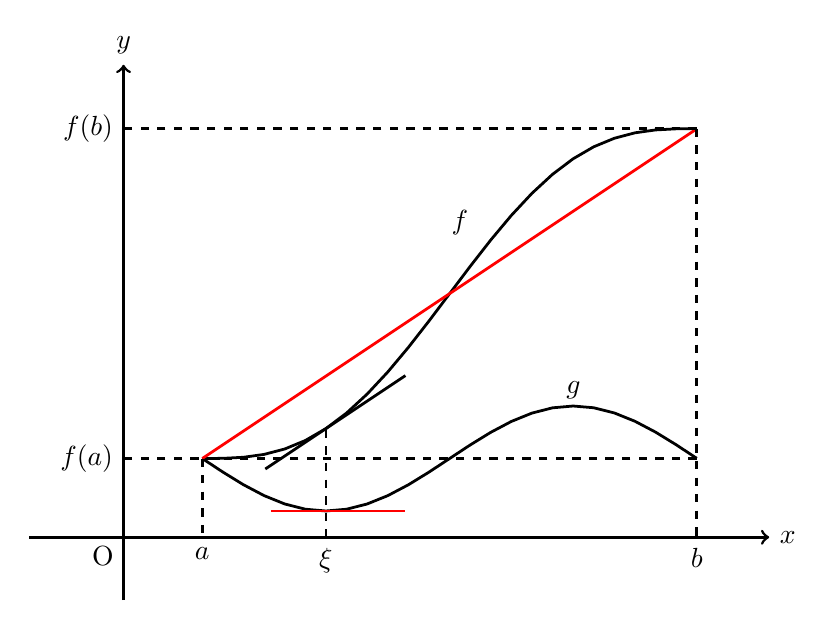
\begin{tikzpicture}[domain=0:8]          
        % 画坐标系
        \draw[line width=1pt, ->] (-1.2,0) -- (8.2,0) node[right] {$x$};
        \draw[line width=1pt, ->] (0,-1.2/1.5) -- (0,9/1.5) node[above] {$y$};
        \draw (0, 0) node[below left] {O};
        
        % f = x + sin
        \draw[line width=1pt, domain=1:7.28] plot (\x, {(1.5 - sin((\x - 1) r) + (\x - 1))/1.5});
        \draw (4.5, 6/1.5) node[left] {$f$};
        
        % g = sin
        \draw[line width=1pt, domain=1:7.28] plot (\x, {(1.5 - sin((\x - 1) r))/1.5});
        \draw (5.5, 2.8/1.5) node[right] {$g$};
        
        % 切线
        \draw[line width=1pt, color=red] (1.87, 0.5/1.5) -- (3.57, 0.5/1.5);
        \draw[line width=1pt, domain=1.8:3.58] plot (\x, {(\x - 0.5)/1.5});
        
        % 辅助线及各种记号
        \draw[line width=1pt, color=red] (1, 1.5/1.5) -- (7.28, 7.78/1.5);
        \draw[line width=1pt, dashed] (2.57, 2.047/1.5) -- (2.57, 0) node[below] {$\xi$};
        \draw[line width=1pt, dashed] (7.28, 7.78/1.5) -- (7.28, 0) node[below] {$b$};
        \draw[line width=1pt, dashed] (7.28, 7.78/1.5) -- (0, 7.78/1.5) node[left] {$f(b)$};
        \draw[line width=1pt, dashed] (1, 1.5/1.5) -- (1, 0) node[below] {$a$};
        \draw[line width=1pt, dashed] (7.28, 1.5/1.5) -- (0, 1.5/1.5) node[left] {$f(a)$};
    \end{tikzpicture}    
    
    }           
\end{document}    
